\clearpage
\section{模糊聚类算法划分居民区域}
\subsection{区域划分聚类步骤}
为提高配送站点的配送效率,前提是要合理划分同城配送区域,确定最集中的配送中心点。

\begin{enumerate}
    \item 选择\rm{k}个初始中心点,例如\rm{c[0]=data[0]}, $\cdots$ \rm{c[k-1]=data[k-1]};
    \item 对于$data[0]$ $\cdots$ $data[n]$, 分别与$c[0]$ $\cdots$ $c[k-1]$比较,假定与$c[i]$差值最少,就标记为$i$;
    \item 对于所有标记为$i$点,重新计算$c[i]=$ \{所有标记为$i$的$data[j]$之和\}标记为$i$的个数;
    \item 重复(2)(3),直到所有$c[i]$值的变化小于给定阈值。
\end{enumerate}

K-Means算法简单易行、便于理解和操作,不但能够处理大规模的聚类问题,对本文研究的同城配送区域划分也有很好的应用效果。算法的聚类数k可以根据经验设定,也可以根据聚类分析对象的数据特征来设置。根据初次聚类的结果进行迭代更新,通过不断的迭代使结果不断接近判断标准,最终聚类结果达到目标标准,聚类中心不再发生变化,算法停止输出结果。

 \begin{figure}[h]
     \centering
     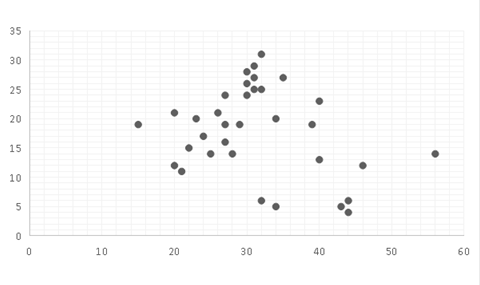
\includegraphics[width=0.5\textwidth]{fig3/fig31.png}
     \caption{居民区的散点分布经经纬度标准化后的散点图}
     \label{fig:my_label}
 \end{figure}
\FloatBarrier
\subsection{居民点的区域划分模型}
\par 本文将案例中需求点的经纬度信息转化为平面坐标,便于使用\rm{K-Means}算法进行求解。用需求点之间距离的大小代表不同需求点之间的相似性,距离越小代表相似性越大。将不同需求点之间的相似性作为划分配送区域的依据,将相似性大的需求点划分到同一个配送区域。为方便后续使用遗传算法对配送路径优化模型进行求解,将地理位置的经纬度信息转化为平面坐标。

\begin{figure}[h]
     \centering
     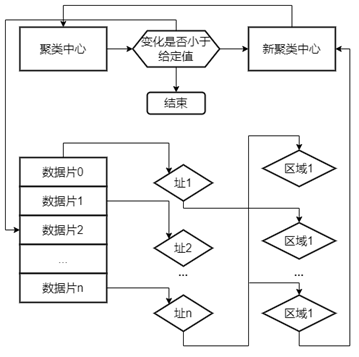
\includegraphics[width=0.5\textwidth]{fig3/fig32.png}
     \caption{K-means算法流程}
     \label{fig:my_label}
 \end{figure}
\FloatBarrier
算法的运行时间随着节点数量的变大而不断减小,这说明对模糊K-Means的并行化切实提升了算法的运行速度,算法具有较好的扩展性。通过模糊K-Means算法根据需求点的实际位置对配送区域进行划分,对聚类效果进行评价确定最佳聚类数为$n$,将$k$值设定为$n$,将配送区域化分为若干部分。

\begin{figure}[h]
     \centering
     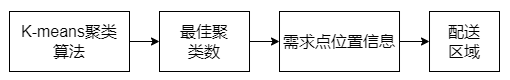
\includegraphics[width=0.5\textwidth]{fig3/fig33.png}
     \caption{K-means算法求解最佳配送区域过程}
     \label{fig:my_label}
 \end{figure}
\FloatBarrier
采用模糊K-Means聚类算法,根据订单需求点的地理位置,确定最佳聚类数,将订单划分到不同的配送区域,得到满足实际配送要求的最佳聚类结果。

\subsection{居民点的区域可视化}
根据上面所述,对区县中的居民点的散点进行统一整合。如下图3-4宁波市各个区县级的地域分布图。其中图中红色、蓝色、绿色区域分别表示鄞州区、海曙区和江北区,灰色区域表示其他区县地区。
\begin{figure}[h]
     \centering
     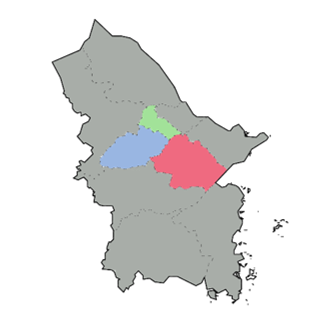
\includegraphics[width=0.3\textwidth]{fig3/fig34.png}
     \caption{宁波地理位置分布图}
     \label{fig:my_label}
\end{figure}
\FloatBarrier
  
根据数据进行统计对区县中的居民点的散点进行分析地址统计,整合出大概地址后,可在地图上二维呈现出散点图状。如下图3-5宁波市中心部分居民区散点分布图。其中由于小区居民散点过多,显示的红点为主要的大集中居民区点。
\begin{figure}[h]
     \centering
     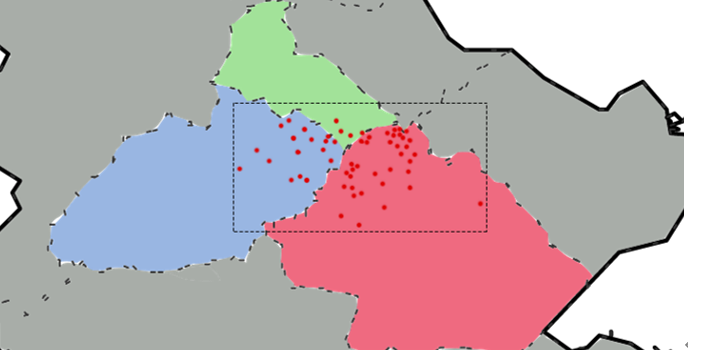
\includegraphics[width=0.5\textwidth]{fig3/fig35.png}
     \caption{宁波市中心部分居民区散点分布图}
     \label{fig:my_label}
\end{figure}
\FloatBarrier
 同时将居民点位置提取出来后,对居民点的具体地址的经纬度进行标准化等处理后,将便可对居民区的位置进行后续分析。
